\section{Implementación}

Los diferentes algoritmos han sido implementados en C++23, para mayor \textit{performance}. Sin embargo, la limitación de éste lenguaje es que el entero máximo que puede albergar es usando 64 bits, es decir, $2^64 \approx 1.8 \times 10^19$.\\
\\
Para la realización de las pruebas en Python, se ha usado \href{https://github.com/pybind/pybind11}{pybind11} para generar módulos de Python a partir del código de C++.

\subsection{Test funcionales}
Para comprobar el correcto funcionamiento de los algoritmos implementados, se han llevado a cabo una batería de tests, tanto para verificar que los resultados obtenidos son correctos, como para poder evaluar el rendimiento de ejecución para diferentes tamaños de números

Con estos test lo que se busca es probar que el algoritmo desarrollado funciona correctamente para ello se ha prubado a ejecutar con números que previamente se conoce si son primos o no. En todos los casos se han obtenido resultados correctos por lo que se puede concluir que funciona correctamente
\begin{figure}[H]
	\makebox[\textwidth][c]{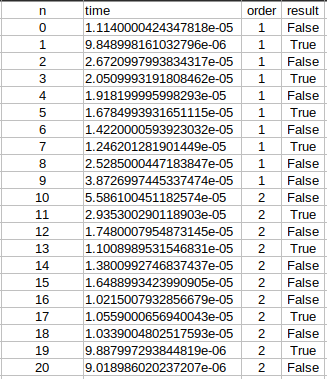
\includegraphics[width=5cm]{img/fucntional_test.png}}
\end{figure}
